\documentclass[xcolor=table]{beamer}
\usetheme{CambridgeUS}
\usecolortheme{beaver}
\useinnertheme{circles}
\useoutertheme{smoothbars}
% \usefonttheme{professionalfonts}

\usepackage[UTF8, heading]{ctex}                                        % for using Chinese
\graphicspath{{../Figures/pdf}{../Figures/png}{../Figures/jpg}}         % set the path where the figures to be searched
\bibliographystyle{apalike}                                             % for brief reference
\usepackage{tdclock}                                                    % for using javascript etc dynamic

\makeatletter
\AtBeginPart{
    \addtocontents{toc}{\protect\beamer@partintoc{\the\c@part}{\beamer@partnameshort}{\the\c@page}}     % for using part in table of contents

    \begin{frame}{Part Outline}
        \partpage
    \end{frame}
}
\AtBeginSection[]{
    \begin{frame}{Section Outline}
        \tableofcontents[currentsection]
    \end{frame}
}
\AtBeginSubsection[]{
    \begin{frame}{Subsection Outline}
        \tableofcontents[currentsubsection]
    \end{frame}
}
% for using part in table of contents
\providecommand\beamer@partintoc[3]{%
  \ifnum\c@tocdepth=-1\relax
    % requesting onlyparts.
    \makebox[6em]{PART #1:} #2
    \par
  \fi
}
\define@key{beamertoc}{onlyparts}[]{%
  \c@tocdepth=-1\relax
}
\makeatother

\title[SlidesHowTo]{Latex Slides How To}
\subtitle[beamer]{How to use beamer}
\author[wjb]{dadadadawjb}
\institute[SJTU]{Shanghai Jiao Tong University}
\date{\today}
\titlegraphic{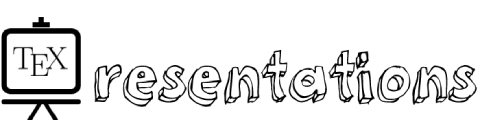
\includegraphics[scale=0.5]{BeamerLogo.png}}
\subject{Slides with Latex}
\keywords{Beamer, HowTo, Latex, Slides}
\logo{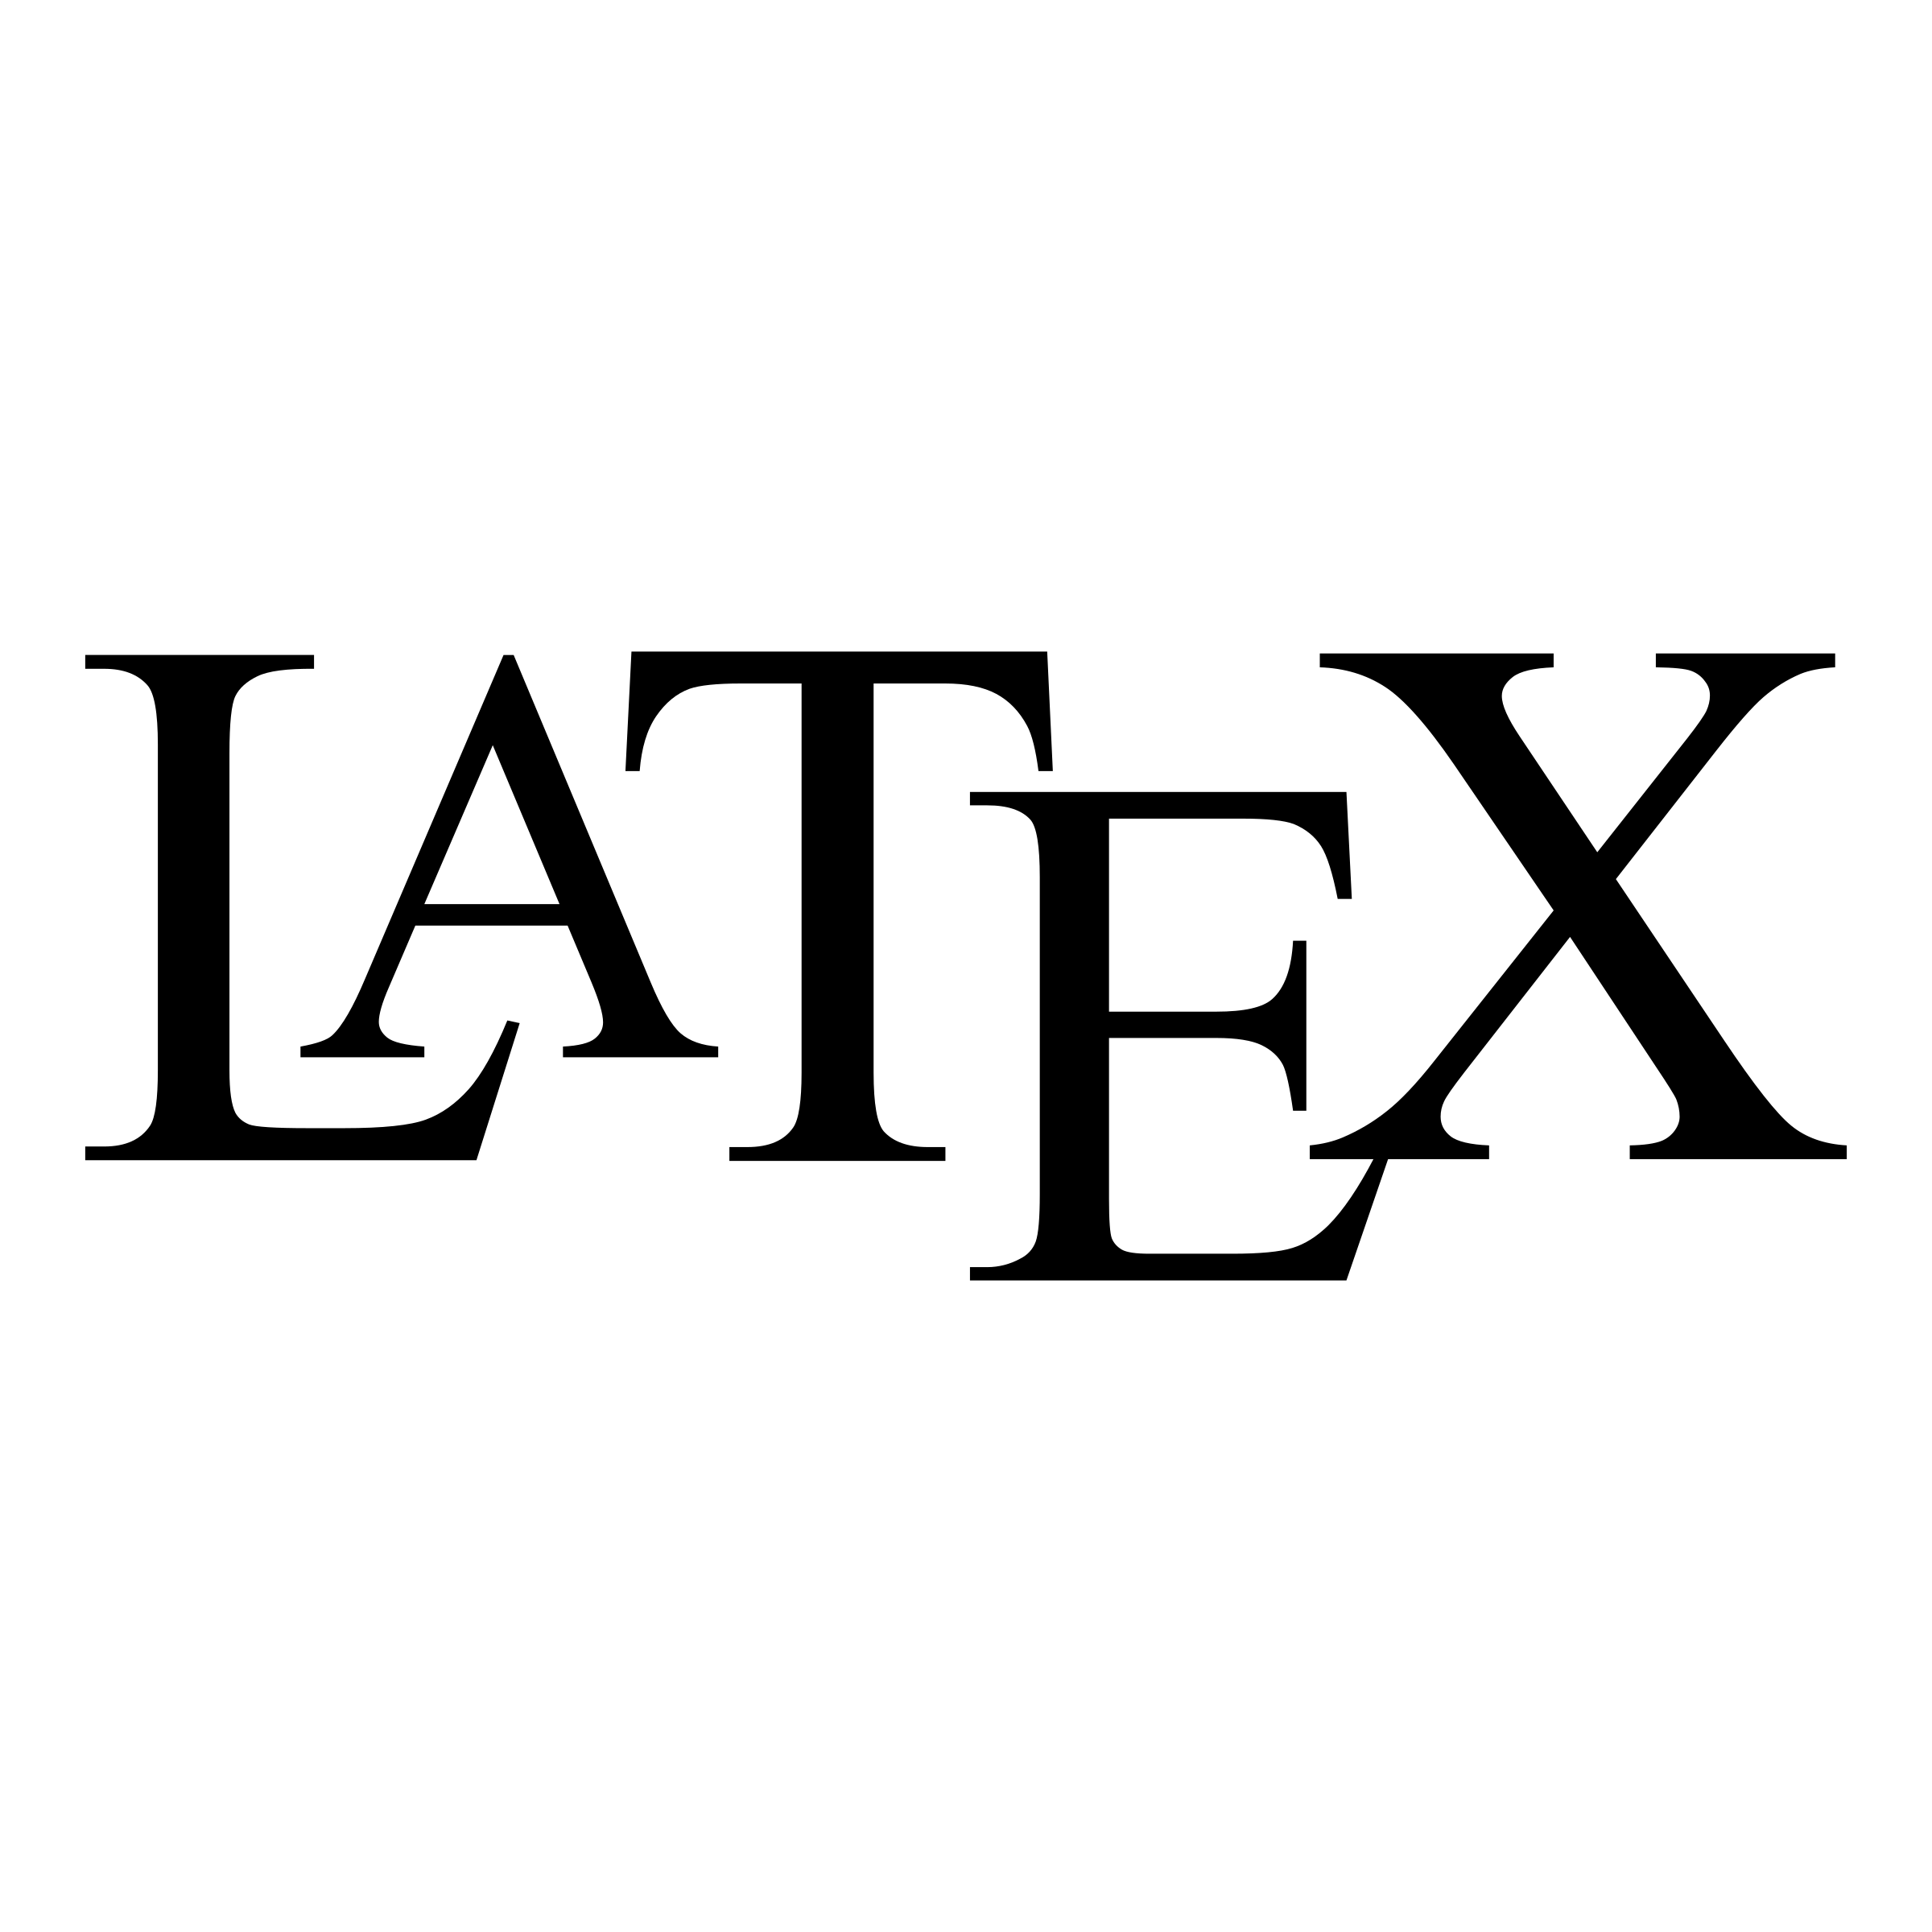
\includegraphics[scale=0.02]{LatexLogo.png}}

\begin{document}
    % title
    \begin{frame}
        \thispagestyle{empty}
        \titlepage
    \end{frame}

    % TOC
    \begin{frame}{Table of Contents}
        \addtocounter{framenumber}{-2}
        \tableofcontents[onlyparts]
    \end{frame}

    \part{First Part}
    \section{Basic Section}
    \subsection{Fundamental}
    \begin{frame}{Frame Title}{Frame Subtitle}
        % \frametitle{Frame Title}
        % \framesubtitle{Frame Subtitle}

        \pause
        Hello, world!

        \pause
        Hello, world!

        \pause
        Hello, world!
    \end{frame}

    \subsection{Animations}
    \begin{frame}{Animations}{onslide}
        \onslide<1>{Only in the first step.}

        \onslide<2->{In and after the second step.}

        \onslide<1, 3>{In the first and third steps.}
    \end{frame}

    \begin{frame}{Animations}{only}
        Counter: \only<1>{1}\only<2>{2}\only<3>{3}\only<4>{4}\only<5->{5}

        \only<5>{Done!}
    \end{frame}

    \begin{frame}{Animations}{list}
        \begin{itemize}
            \item<1-> The first item.
            \item<3-> The last item.
            \item<2-> Then this.
        \end{itemize}

        \begin{enumerate}[<+->]
            \item The first item.
            \item The second item.
            \item The third item.
        \end{enumerate}
    \end{frame}

    \begin{frame}{Animations}{emphasize}
        \structure{emphasize}

        \alert{emphasize}

        \begin{enumerate}
            \item<+-> The first item.
            \item<+-| alert@+> The second item.
            \item<+-> The third item.
        \end{enumerate}
    \end{frame}

    \subsection{Block}
    \begin{frame}{Theorems}
        \begin{theorem}<1->[Moore's Law]
            The number of transistors in a dense integrated circuit (IC) doubles about every two years.
        \end{theorem}
        
        \begin{corollary}<2->[CS Law]
            It is pretty awesome to learn Computer Science!
        \end{corollary}

        \begin{proof}<3->
            It is obvious. \qedhere % it may be error, so we can explicitly add this to show the symbol
        \end{proof}
    \end{frame}

    \begin{frame}{Statements}
        \begin{definition}<1->[Computer Science]
            A pretty awesome discipline!
        \end{definition}

        \begin{example}<2->
            Operating System, Computer Architecture, Computer Organization, Computer Networks, etc.
        \end{example}

        \begin{fact}<3->
            So many people love computer science!
        \end{fact}
    \end{frame}

    \begin{frame}{Blocks}
        \begin{block}<1->{Block Title}
            This is a normal block.
        \end{block}

        \begin{alertblock}<2->{Alertblock Title}
            This is an alert block.
        \end{alertblock}

        \begin{exampleblock}<3->{Exampleblock Title}
            This is an example block.
        \end{exampleblock}
    \end{frame}

    \section{Dynamic}
    \subsection{Animations}
    \newdimen\xoffset
    \begin{frame}{Animations}{animate}
        \animate<2-10>
        \animatevalue<1-10>{\xoffset}{0cm}{5cm}
        \hspace{\xoffset} Hello, world!
    \end{frame}

    \begin{frame}{Animations}{transformation}
        % only in full screen mode
        \begin{itemize}[<+->]
            \small
            \item Hello, world!
            \item Hello, world!
            \item Hello, world!
            \item Hello, world!
            \item Hello, world!
            \item Hello, world!
            \item Hello, world!
            \item Hello, world!
            \item Hello, world!
            \item Hello, world!
            \item Hello, world!
            \item Hello, world!
            \item Hello, world!
            \item Hello, world!
            \item Hello, world!
        \end{itemize}

        \transblindshorizontal<1>
        \transblindsvertical<2>
        \transboxin<3>
        \transboxout<4>
        \transcover<5>
        \transuncover<6>
        \transdissolve<7>
        \transfade<8>
        \transglitter<9>
        \transpush<10>
        \transwipe<11>
        \transsplithorizontalin<12>
        \transsplithorizontalout<13>
        \transsplitverticalin<14>
        \transsplitverticalout<15>
    \end{frame}

    \subsection{Multimedia}
    % bug exists

    % \begin{frame}{Multimedia}{movie}
    %     \movie[width=4cm, height=3cm]{Click to play}{Movie.mp4}
    % \end{frame}

    % \begin{frame}{Multimedia}{audio}
    %     \sound[autostart]{}{Audio.au}
    % \end{frame}

    \subsection{Javascript}
    \begin{frame}{Javascript}{tdclock}
        % must usepackage tdclock, bug exists
        current time: \tdtime; passed time: \crono
    \end{frame}

    \part{Second Part}

    \begin{frame}{Literature Reference}
        \nocite{dellaert2021neural}
        \nocite{Tewari20eurographics_neural_rendering}
        \nocite{Mildenhall20eccv_nerf}
        \bibliography{LiteratureReference.bib}
    \end{frame}
\end{document}